\subsection{Prelimiary to Resistor Capacitor Circuits}

This will be brief. I assume that most of the readers are reasonably comfortable with complex exponential already, and that Laplace Transforms are not unfamiliar either. Almost exclusively basing myself on the textbook. 

\subsubsection{Complex Exponentials}

All solutions to linear homogeneous equations are of the form $e^{st}$ where $s$ is a \textit{complex number}.

\begin{equation}
    s = \sigma + j\omega = M cos(\phi) + j M sin(\phi)
\end{equation}

where $j = \sqrt{-1},\ \sigma$ is the real part of the complex number and $\omega$ os the imaginary part. M represents its \textit{magnitude} and $\phi$ its phase. Magnitude and phase of a complex number obey the following relationships: 

\begin{equation}
    M = \sqrt{\sigma^2 + \omega^2}\\
\end{equation}
\begin{equation}
    \phi = \mathrm{arctan} (\frac{\omega}{\sigma})
\end{equation}
The magnitude of a complex number $s$ is often denoted as $|s|$. Furthermore,
applying the properties of complex exponentials, one can observe that:
\begin{equation}
    e^{j\phi} = cos(\phi) + j sin(\phi)
\end{equation}
\begin{equation}
    e^{-j\phi} = cos(\phi) - j sin(\phi)
\end{equation}
it follows that $s$ can also be written as: 
\begin{equation}
    s = Me^{j\phi}
\end{equation}
\textbf{These notations can be used to solve higher order differential equations.} As an example, we consider the second order linear homogeneous equation: 
\begin{equation}
    \frac{d^2}{dt^2}V + \alpha \frac{d}{dt}V + \beta V = 0
\end{equation}
Assuming $e^{st}$ is an \textit{eigenfunction}\footnote{An eigenfunction is a nonzero solution of a second order linear homogenous differential equation} and substitute for V: 
\begin{equation}
    s^2e^{st} + \alpha se^{st} + \beta e^{st} = 0
\end{equation}
Solving for $s$ we obtain
\begin{equation}
    s = \frac{-\alpha \pm \sqrt{\alpha^2 -4\beta}}{2}
\end{equation}
Consequently, if $\alpha^2 -4\beta \geq 0$, $s$ is real, otherwise it is complex. 

\subsection{Step and Delta function}

If you do not know what this is, please see Textbook Linear Systems Chapter in appendix, section 8.3 and 8.4.

\subsubsection{The Heaviside-Laplace Transform}

By analyzing the example of the previous section we can make
the following observation: Any time we substitute the eigenfunction $e^{st}$ into a
linear differential equation of order $n$, the following property obtains:
\begin{equation}
    \frac{d^n}{dt^n}e^{st} = s^ne^{st}
\end{equation}

\textbf{In other words: We can consider $s$ as an operator meaning \textit{derivative} with respect to time. Similarly, we can view $\frac{1}{s}$ as the operator of \textit{integration} with respect to time (Oliver Heaviside)}

Formally, we write; 

\begin{equation}
    \mathscr{L}\{y(t)\}=Y(s)= \int_{-\infty}^{\infty} {y(t)e^{-st}} dt
\end{equation}
Notice that we write $y(t)$ for a signal in \textit{time domain} and $Y(s)$ for a signal in \textit{Laplace domain}. A signal in laplace domain is simply a signal in time domain which we have applied the Laplace transformation to (equation above). If you don't understand this, don't worry, figuring out how this works in practice is all that matter.  

\subsubsection{Transfer Function}

Technically, to understand properly the concept of a transfer function, you should know what convolution, impulse response and Laplace transforms (more than what I introduced) are all about. But let's just make things very simple and say that we define the transfer function $H(s)$ as follows: 
\begin{equation}
    H(s) \equiv \frac{Y(s)}{X(s)}
\end{equation}

which underlies very complex ideas just to say that it's the output divided by the input \textbf{both in Laplace domain} (see Figure \ref{fig:Linear_Systems_Laplace}).

\begin{figure}[H]
    \centering
    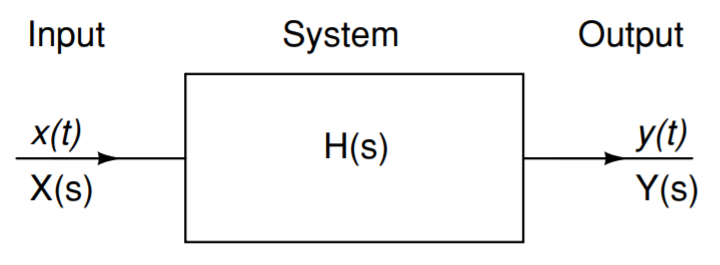
\includegraphics[width=0.5\linewidth]{../../Figures/Input_Output_Laplace.PNG}
    \caption{Typical black-box representation of a linear system. Its input is the signal $x(t)$ in time domain, and $X(s)$ and its output is the signal $y(t)$ in time domain and $Y(s)$ in Laplace domain. Adapted from textbook}
    \label{fig:Linear_Systems_Laplace}
\end{figure}
